\chapter{Conclusioni}\label{cap:conclusioni}
\section{Conclusioni}\label{sez:conclusioni}
Questo studio, ha cercato di rispondere alla domanda: "Cos'\`e Blazor?".
A tal fine, \`e stato descritto prima di tutto quale sia il contesto che ha portato alla creazione di questo framework, che sfruttando varie tecniche e strumenti permette anche agli sviluppatori web backend di avvicinarsi al frontend senza dover necessariamente imparare ed utilizzare Javascript.
Si \`e poi descritto quali siano le tecnologie utilizzate da questo framework e come in parte siano differenti a seconda del modello scelto.
\`E stata descritta un'applicazione web implementata per questo lavoro di tesi sfruttando Blazor Server, e quando presenti sono stati citati gli esempi messi a disposizione per gli altri modelli.
Tutto ci\`o \`e stato utilizzato poi per spiegare il diverso funzionamento, con pro e contro, tra i due principali modelli disponibili in questo momento, ovvero Blazor Server e Blazor WebAssembly. 

\begin{figure}[H]
	\centerline{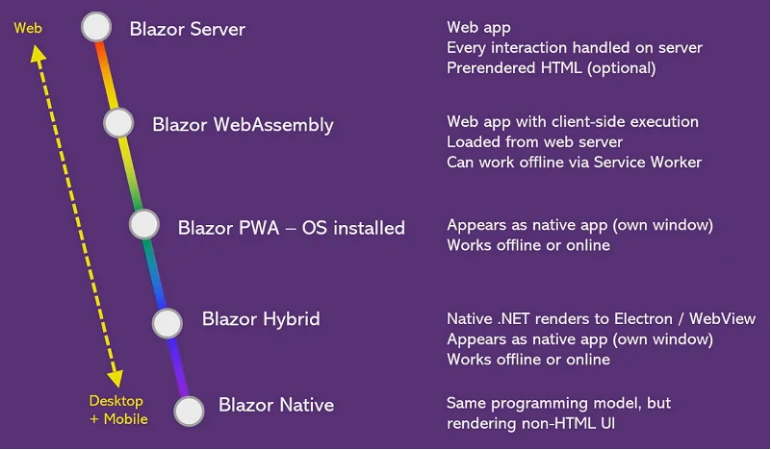
\includegraphics[scale=0.5]{figure/BlazorModels.PNG}}
	\caption{Modelli Blazor}
	\label{fig:blazorModels}
\end{figure}

In figura \ref{fig:blazorModels} \`e presente il riepilogo di tutti i modelli Blazor, presenti e futuri.
La direzione del framework, nato per lo sviluppo web, \`e chiara: gli sviluppi futuri saranno orientati al client(Mobile e Desktop) per permettere agli sviluppatori di raggiungere pi\`u piattaforme e di sviluppare tipologie di applicazioni molto diverse, offrendo per\`o un'esperienza di sviluppo costante, aumentando la produttivit\`a degli sviluppatori.

Da questo studio \`e infatti emerso che non esiste una scelta di default sempre corretta, poich\'e a seconda delle esigenze dell'applicazione da sviluppare lo stesso modello pu\`o risultare pi\`u o meno adatto.

Quando si vuole sviluppare applicazioni per le quali:
\begin{enumerate}
	\item \`E necessario che il codice non lasci mai il server, quindi dove la sicurezza delle logiche di business ha la massima priorit\`a;
	\item Si \`e certi che gli utenti dovranno utilizzare l'applicazione avranno accesso costantemente una connessione stabile;
	\item Si hanno a disposizione risorse in modo sufficiente(RAM e CPU) sulla macchina che ospiter\`a l'applicazione, e le risorse utilizzabili si possono aumentare durante eventuali picchi di utenti connessi in modo concorrente o al crescere della complessit\`a della UI dell'applicazione sviluppata;
	\item Si vuole utilizzare Blazor per sviluppare e si ha la necessit\`a di iniziare lo sviluppo il prima possibile;
\end{enumerate}

La scelta migliore tra i modelli Blazor, \`e Blazor Server.

Questo primo modello, essendo anche il pi\`u maturo, \`e gi\`a una valida tecnologia da tenere in considerazione e sfruttare quando risulta adatto.
Per ora \`e comunque sconsigliato utilizzare questa tecnologia senza conoscere affatto JS, dato che in alcuni casi potrebbe essere necessario utilizzarlo, come \`e successo durante lo sviluppo di BlazorPong.

Per il resto delle applicazioni, probabilmente \`e pi\`u adatto l'utilizzo di Blazor WebAssembly.

\`E importante ricordare che durante lo sviluppo di BlazorPong, quasi ad ogni aggiornamento di versione di Blazor Server, che era ancora in preview, ci sono state breaking changes per le quali \`e stato necessario riscrivere parzialmente l'applicazione, ma da quando si \`e raggiunta una release stabile, il processo di update \`e stato quasi indolore e le novit\`a introdotte largamente retrocompatibili.

Blazor WebAssembly ad ogni modo \`e il modello pi\`u interessante in questo momento, perch\`e architetturalmente \`e il pi\`u simile ai framework maggiormente utilizzati dagli sviluppatori web frontend, ma permette di non essere costretti ad utilizzare esclusivamente JS per la parte dinamica del codice dell'applicazione web che si vuole sviluppare, punto estremamente importante per gli sviluppatori che utilizzano tecnologie Microsoft.

Inoltre utilizzando la compilazione AOT verso WebAssembly, un'applicazione scritta con Blazor WebAssembly potrebbe arrivare ad avere prestazioni  migliori di un'applicazione equivalente, scritta utilizzando JS.

I problemi del modello WebAssembly per\`o sono evidenti:
\begin{enumerate}
	\item Le prestazioni native che potenzialmente potrebbero essere raggiunte, sono ancora lontane in questo momento.
	Questo principalmente perch\`e il codice convertito in WebAssembly \`e solo il runtime Mono che quindi interpreta il codice compilato dell'applicazione durante l'esecuzione(le DLL) e non ha le prestazioni native che Blazor potrebbe raggiungere.
	Se Microsoft riuscir\`a a implementare un compilatore che esegua direttamente la compilazione di tutto il codice da C\# a WebAssembly, allora le prestazioni del codice potrebbero rispettare ci\`o che il framework cerca di offrire, tuttavia molto dipender\`a dall'efficienza di questo nuovo compilatore;
	\item Il tooling messo a disposizione non \`e sufficiente per giustificare l'utilizzo di Blazor in produzione, dato che nemmeno il debugging al momento risulta pienamente supportato;
	\item Alcuni eventi della UI, non sono ancora supportati da Blazor, che fornisce delle interfacce per essere interoperabile con JS, ma di fatto non ne elimina ancora l'obbligo della conoscenza, principale motivo per il quale un developer potrebbe volerlo utilizzare.
	\item La community, essendo nata solo di recente, non \`e paragonabile a quella di JS e dei suoi maggiori framework, quindi il supporto, gli esempi disponibili online come anche la documentazione e gli effettivi utilizzatori, sono molto limitati, almeno per ora.
\end{enumerate}

Infine Blazor PWA, Blazor Hybrid e Blazor Native al momento sono progetti altamente sperimentali, ed il loro utilizzo a scopo non puramente accademico potrebbe rivelarsi una scelta sbagliata, il consiglio \`e quello di tenerli in considerazione quando verranno rilasciati ufficialmente ed eventualmente di valutare se effettivamente il loro utilizzo sia giustificato.

Il presente studio prova quindi ad aggregare e studiare le informazioni disponibili al momento su Blazor, ed \`e importante tenere presente che solo uno dei 5 modelli attualmente annunciati \`e stato ufficialmente rilasciato, quindi alcune delle cose descritte potrebbero cambiare nel tempo, come ad esempio le tecnologie sulle quali si basano Blazor PWA o Blazor Hybrid.

Una raccomandazione per ulteriori ricerche future potrebbe essere quella di realizzare uno studio simile per determinare eventuali differenze ed evoluzioni siano avvenute nel tempo a Blazor rispetto a quello qui descritto ed i motivi di questi cambiamenti, confrontandolo poi con framework con lo stesso scopo ma non prodotti da Microsoft.
Un'altro punto di partenza potrebbe essere quello di effettuare indagini su quanti developer backend e frontend abbiano scelto o scartato Blazor e per quali motivi lo abbiano fatto.